
\section{Introducción}
\label{sec:introduccion}
\setlength{\parskip}{1em} % Ajusta el valor según prefieras

En la actualidad, la sociedad concede una importancia creciente al bienestar integral \cite{bib:noticia2024ipmark}, donde la salud mental ocupa un lugar tan relevante como la salud física. Nuestra vida cotidiana está cada vez más influenciada por la digitalización y un ritmo acelerado que, si bien ofrece numerosas ventajas, también puede generar estrés, ansiedad y una desconexión con nuestro estado emocional interno \cite{bib:articulo2025tecnoestres}. Este contexto ha generado nuevas oportunidades y desafíos en ámbitos como la salud digital, el desarrollo de software orientado al usuario y las ciencias del comportamiento. 

Esta transformación representa una tendencia macroeconómica cuya magnitud se evidencia en las proyecciones del mercado global de la salud y el bienestar. Se estima que dicho sector pasará de una valoración de 6.521,92 miles de millones de dólares en 2026 a superar los 10.381,4 miles de millones para el año 2035, manteniendo una tasa de crecimiento anual compuesto (CAGR) del 5,3\% \cite{bib:business_research_wellness}, tal y como ilustra la proyección cronológica de la Figura \ref{fig:mercado_bienestar}.

\begin{figure}[H]
    \centering
    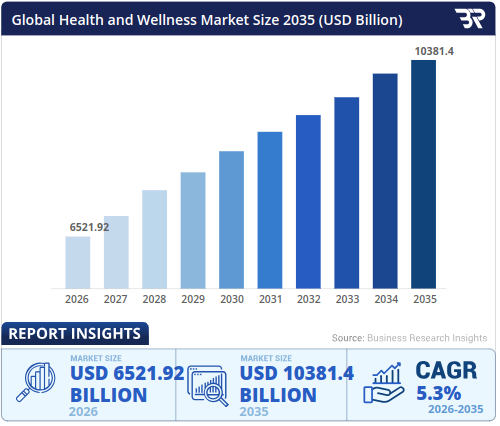
\includegraphics[width=0.65\textwidth]{Imagenes/mercado_bienestar.png}
    \caption{Proyección del tamaño del mercado mundial de la industria de la salud y el bienestar 2026-2035 \cite{bib:business_research_wellness}.}
    \label{fig:mercado_bienestar}
\end{figure}

Uno de los principales retos actuales es la falta de autoconocimiento emocional sistemático y basado en datos, con esto nos referimos a la capacidad de analizar el bienestar emocional utilizando registros objetivos y cuantificables, en lugar de depender únicamente de la memoria retrospectiva, la cual es a menudo imprecisa ya que no siempre se recuerda todo. Este desafío afecta a un amplio espectro de la población, desde jóvenes hasta adultos, y se manifiesta en la dificultad para identificar patrones anímicos, comprender las causas de sentimientos recurrentes o simplemente recordar cómo nos hemos sentido en un período determinado. Abordar esta problemática resulta esencial, ya que una mayor conciencia emocional está directamente relacionada con una mejor toma de decisiones, una mayor resiliencia psicológica y una gestión más eficaz del estrés diario \cite{goleman2004leader}.


En los últimos años, la incorporación de tecnologías de sensores \textit{wearables} ha supuesto una transformación significativa, creando un mercado global multimillonario y cambiando la forma en que los usuarios monitorizan sus condiciones de salud. Esta tendencia se ha normalizado a través de \textit{smartwatches} y pulseras de actividad, que integran en la vida diaria el registro de datos biométricos. Estos dispositivos utilizan sensores avanzados para medir los niveles de estrés. Estas innovaciones de \textit{hardware} han impulsado la creación de potentes ecosistemas de \textit{software} que permiten a los usuarios cuantificar y visualizar su salud y demuestran el potencial de la ingeniería de \textit{software} para mejorar la introspección y el cuidado personal \cite{perez2021recent}. Sin embargo, este registro automático de datos físicos no cubre una parte fundamental del bienestar: el estado emocional subjetivo, el cual no se puede medir con ninguno de estos sistemas ya que requiere un registro manual y contextualizado de la propia persona.

Para cubrir precisamente ese hueco, en este Trabajo Fin de Grado (TFG) se propone el diseño y desarrollo de una aplicación web para el seguimiento diario del estado de ánimo personal, con el fin de proporcionar a los usuarios una herramienta intuitiva y eficaz para el autoconocimiento emocional. El proyecto se centra en crear una plataforma que no solo permita el registro rápido del humor, sino que también facilite la asociación de este con actividades, eventos y otros factores contextuales. De este modo, busca dar respuesta a la necesidad de una herramienta que sea menos clínica que las aplicaciones terapéuticas y más estructurada y visual que un diario tradicional.


Con la realización de este trabajo se pretende ofrecer una solución tecnológica que guíe a los individuos en la gestión de su bienestar mental. Asimismo, el proyecto está dirigido al público general interesado en el crecimiento personal, ofreciendo una solución que mejora la situación actual al centrarse en la visualización de datos y la detección de correlaciones de forma automática, esto significa que el sistema será el encargado de analizar los registros del usuario y revelarle patrones como qué actividades se correlacionan con un mejor ánimo sin que este deba interpretar los datos manualmente).


Por ejemplo, un estudiante universitario que experimenta altos niveles de estrés podría utilizar la aplicación para registrar su estado de ánimo general (ej. un 5/10). A continuación, para dar contexto, seleccionaría \textit{tags} de la paleta genérica, como \texttt{\#Estudios} y \texttt{\#Dormir}. Para que el análisis sea preciso y no básico, la aplicación le permitiría puntuar opcionalmente esos \textit{tags} de forma individual, pudiendo marcar \texttt{\#Estudios} con un 2/10 y \texttt{\#Dormir} con un 6/10. Tras varias semanas, la plataforma podría generar gráficos que revelen una correlación clara, tal y como se simula en el gráfico de la Figura \ref{fig:ejemplo_analisis}: el \textit{tag} \texttt{\#Estudios} tiene una puntuación de impacto promedio de 3.5/10 (la causa del estrés), mientras que un \textit{tag} como \texttt{\#Ocio} mantiene una media de 8.5/10. De esta manera, se busca demostrar la aplicabilidad real de la propuesta y su capacidad para ayudar a los usuarios a tomar decisiones informadas que mejoren su calidad de vida.

\begin{figure}[h!]
    \centering
    \includegraphics[width=0.8\textwidth]{Imagenes/ejemplo_analisis.pdf}
    \caption{Simulación de un gráfico generado por el módulo de análisis de datos de MoodNest, mostrando la puntuación promedio de cada \textit{tag} para el caso del estudiante.}
    \label{fig:ejemplo_analisis}
\end{figure}

En resumen, este TFG tiene como objetivo la creación de una aplicación intuitiva y atractiva, que fomente el hábito del registro diario. De esta manera, los usuarios podrán utilizarla en cualquier momento y lugar, convirtiendo el autoconocimiento emocional en una práctica accesible, eficiente y, en última instancia, transformadora para su bienestar.
